\begin{event}{5th Encuentro Colombiano de Combinatoria}{2016ECCO}{Medellin (Colombia), 2016-06-13 to 2016-06-24}{PS}{130}{http://ecco2016.combinatoria.co/}

\textbf{Main goals.} ECCO is a combinatorics summer school organized every other year in Colombia. It welcomes 
students from all over the world of all levels: from undergraduates to postdocs. It is known to be a very
interesting event and to have a great impact for combinatorics in Colombia and South America in general.
The Sage community in combinatorics being very active, it was a great occasion to introduce Sage
to a new generation of researchers.

\textbf{ODK implication.} Viviane Pons was sent by ODK to give two Sage interventions
during the school.

\textbf{Event summary.} Each intervention was 2 hours long with around 50 participants each time.
Most participants were using the university computers. 50 USB sticks were bought previous
to the conference and set up with bootable Linux and sage, allowing for a very quick setup
during the two sessions without relying on on-line options. The students worked on some
introduction tutorials and also specifically made tutorials in relation with the on-going
classes.  

\textbf{Demographic.} 66 participants came from South and Central America, 34 from North America
and 30 from Europe. 

\textbf{Results and impact.} 
\begin{itemize}
\item The organizers were very happy that ODK would propose to send someone at the school. 
They did not have anyone who could carry such an intervention which requires both Sage and
technical skills.

\item It was quite a challenge to get Sage to work in approximatively 10 minutes for 50
computers all together. The solution of the bootable USB sticks has been developed by Thierry
Monteil but is not well known nor well documented. This was an occasion to test this solution
in this particular setup and improve our experience for future events.

\item The bootable USB keys were very successful and many students brought their own sticks to
get a copy of the software. During the sessions, we could also help students install
Sage on their own computers.

\item Many of the students, especially the younger ones from South America, had never used
Sage before. We proposed many different tutorials so that everyone could have something to
work on and we created exercises related to the class content of the two weeks. We received
 enthusiastic feedbacks for the sessions.

\item Some of the introduction tutorials of the Sage documentation were translated into 
Spanish for the sessions and will eventually be added to Sage.

\item The conference in general was a very rewarding event. It has been growing and successful
for the past ten years with a strong focus on inclusivity and impact. It was a great occasion
to be part of the event and learn from their experience. A blog post from Viviane Pons was
published by the \emph{AMS Blog, On Teaching and learning mathematics}\cite{16PonsECCO}.
\end{itemize}



\begin{figure}[ht]
\caption*{Participants of ECCO at the Sage sessions}
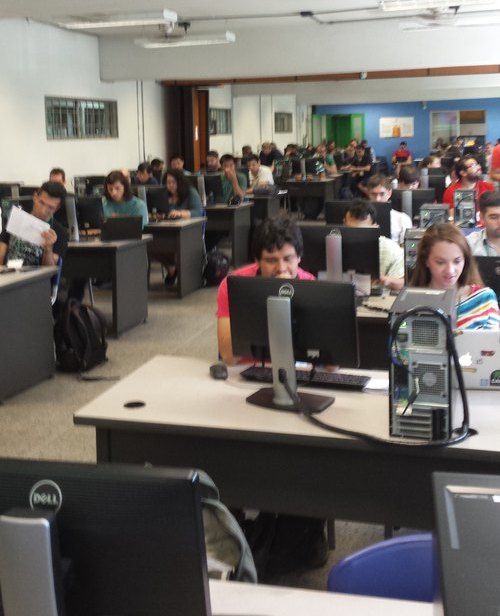
\includegraphics[scale=0.5]{pictures/ECCO-1.jpg}

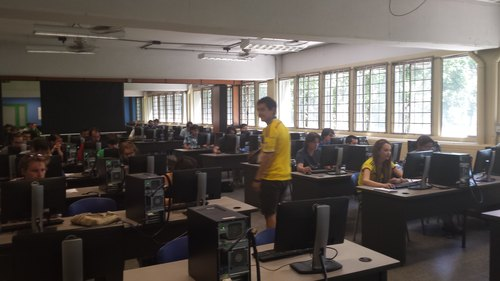
\includegraphics[scale=0.5]{pictures/ECCO-2.jpg}
\end{figure}



\end{event}
